Digital, computer-based real-time systems became widespread rapidly with the availability of microprocessors getting more powerful and cheaper from year to year.

\section{ Introduction}

Real-Time systems, as used in the wide area of automation, have 2 basic requirements,

\begin{enumerate}
	\item  The \textbf{logical correctness} of the systems output as a response to its inputs, and
	\item  The \textbf{timeliness} of the outputs available.
\end{enumerate}


For example, this is obvious for an airbag control, for which a correct decision for ignition is required at the right millisecond, otherwise the resulting behaviour can be harmful !\\

Since there is a "digital revolution" the past few decades, a strong trend to applications with microprocessors and witch microcontrollers particularly can be observed.\\

This means, that classical solutions for \textbf{real-time systems} (e.g. analog controller circuits) are replaced by \textbf{software applications} running on a microprocessor or a microcontroller.\\

Thus, an important part of \textbf{a real-time system is software}. This type of software is much different from commonly used software known from PC applications like office programs, or internet browsers, since real-time requirements have to be met.\\

In the area of real-time software development, the classical C programming language is widely used, due to its outstanding maturity and flexibility, especially with industrial PC applications, or with microcontroller applications.\\

Furthermore there is a need for PLC controls (de: SPS) in industrial automation.\\

Examples for Real-Time Systems

\begin{figure}%
    \centering
    \subfloat[\centering  Automotive Door Contol Unit with Anti-Squeeze ]{{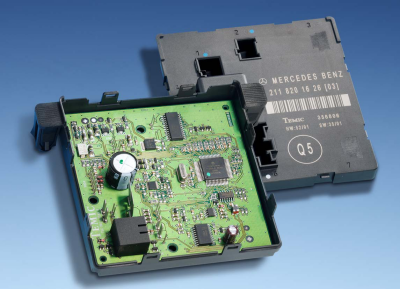
\includegraphics[width=8cm, 		   			height=5.5cm]{Images/image3.png} }}%
    \qquad
    \subfloat[\centering Undistorted image]{{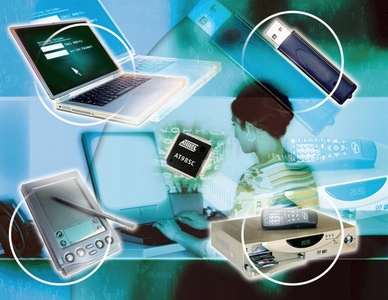
\includegraphics[width=8cm, height=5.5cm]{Images/image4.png} }}%
    \qquad
     \subfloat[\centering Car with $>$ 100 ECUs]{{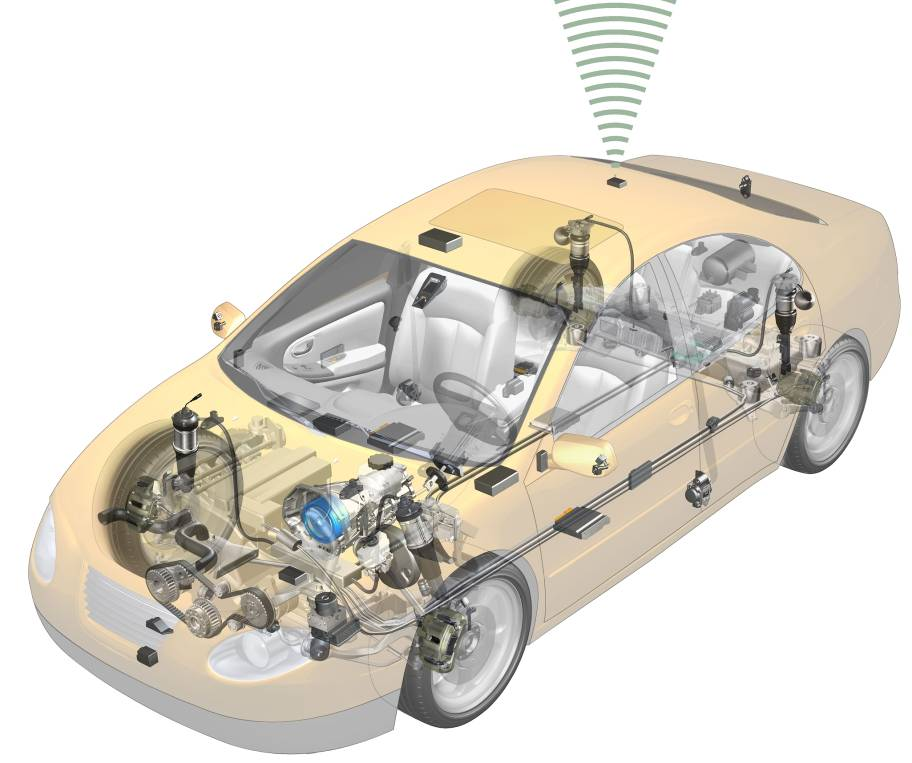
\includegraphics[width=7cm, height=5.5cm]{Images/image5.png} }}%
    \qquad
    \subfloat[\centering Pacemaker]{{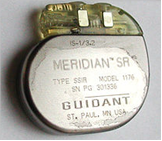
\includegraphics[width=6cm, height=5cm]{Images/image6.png} }}%
    \qquad
     \subfloat[\centering A319 Cockpit]{{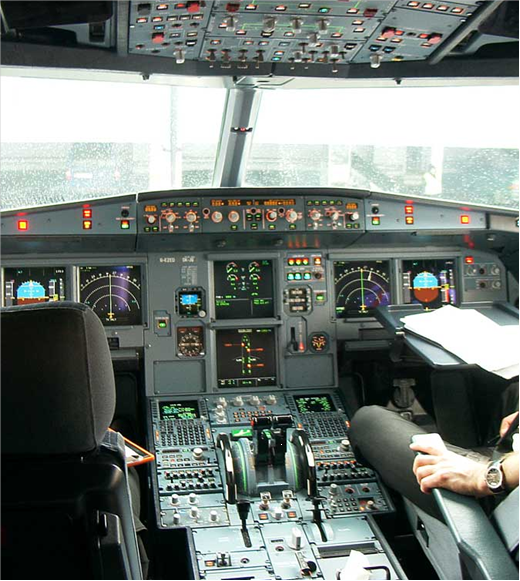
\includegraphics[width=8cm, height=5cm]{Images/image8.png}}}%
    \qquad
    \subfloat[\centering wikipedia.de: Arc welding of metal parts with industrial robots (KUKA). IPC, PLC]{{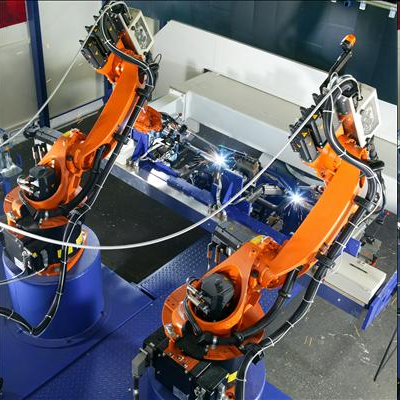
\includegraphics[width=8cm, height=5cm]{Images/image7.png} }}%
    \qquad
    \caption{ Comparison of results of video 1 (checkerboard000)}%
    \label{v1}%
\end{figure}


\begin{itemize}
	\item Examples of the use of real-time systems are found in the following areas: 
	\begin{enumerate}
		\item  Production 
		\item  Aerospace 
		\item  Automotive Electronics
		\item  Medicine
		\item  Military Technology, 
		\item  e-Banking, 
		\item  e-Trading, 
		\item  Telecommunications, 
		\item  Network Management, 
		\item  Power Generation/Management, 
		\item  Navigation
	\end{enumerate}
\end{itemize}

\textbf{The} need for Software\textbf{(mainly C-Code)in all areas of application grows rapidly}. 

\begin{tcolorbox}[colback=blue!5!white,colframe=blue!75!black]
  Moore's Law: “die Anzahl der Transistoren pro Chipfläche verdoppelt sich alle 2 Jahre”
\end{tcolorbox}

\begin{figure}[h]
    \centering
    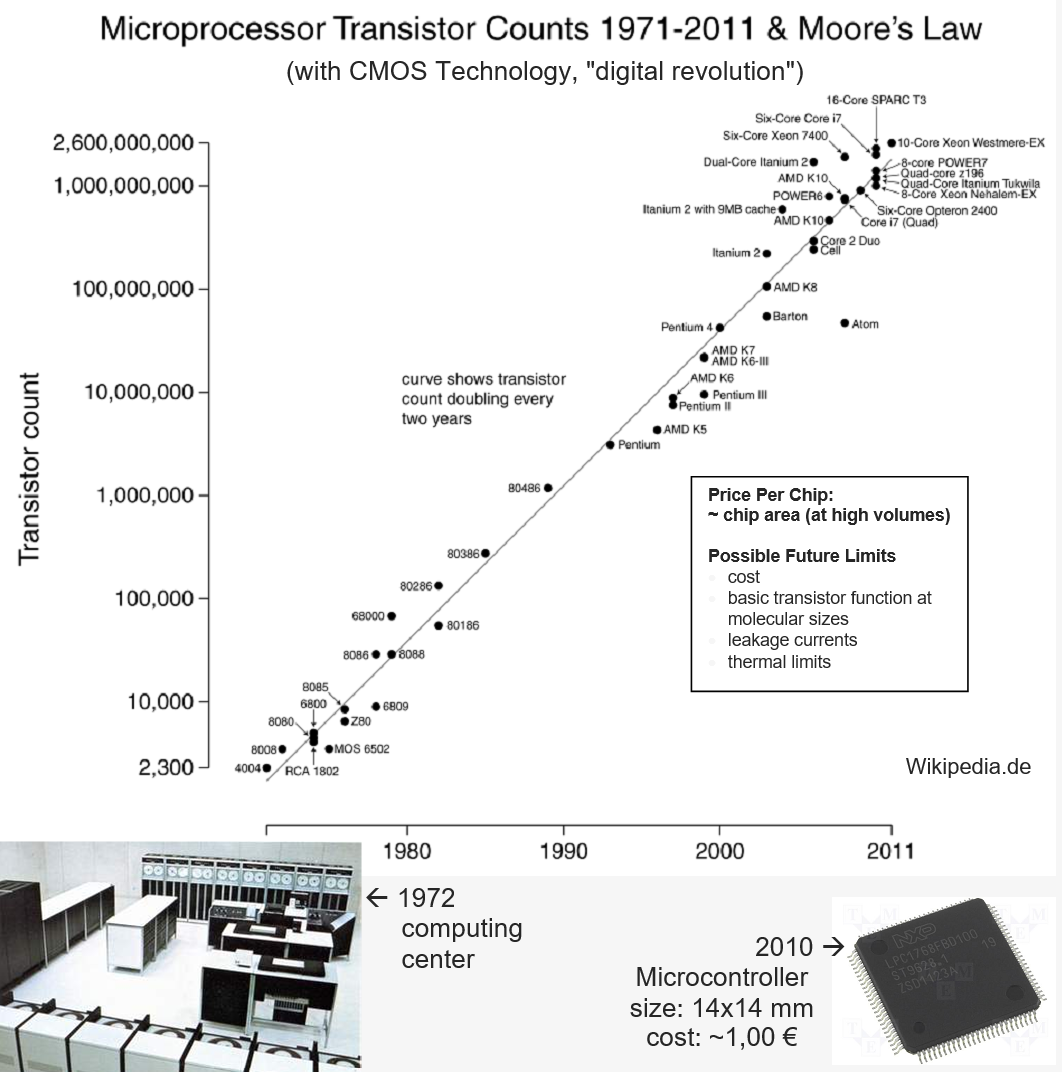
\includegraphics[width=13cm, height=10cm]{Images/image9.png}
    \caption{Moore's Law}
    \label{fig:Fig 3}
\end{figure}

\textbf{ Software for Real-Time Systems} differs substantially from software for generalpurpose computers (PC) due to the \textbf{requirements on the real-time behavior} !\\

Many methods of \textbf{classical software development} of non-real-time systems can not be used due to the lack of predictability.\\

For the development of real-time systems, special methods are required.\\


\section{ Requirements}

\newpage The validity of an operation of a real-time system depends on

\begin{enumerate}
	\item  its logical result, and
	\item  the physical time this result is available
\end{enumerate}

\begin{figure}%
    \centering
    \subfloat[\centering logical correct, but timing incorrect]{{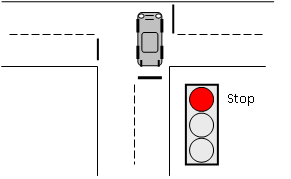
\includegraphics[width=7cm, 		   			height=5cm]{Images/image10.png} }}%
    \qquad
    \subfloat[\centering logical correct, and timing correct]{{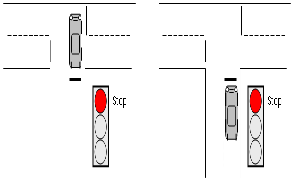
\includegraphics[width=7cm, height=5cm]{Images/image11.png} }}%
    \qquad
    %\caption{ Comparison of results of video 1 (checkerboard000)}%
    \label{fig:Fig 3}%
\end{figure}

\textbf{The traffic light control must determine traffic light phases logically and temporally correct.}\\

For real-time systems, the logical correctness \textbf{and} the timing correctness is required.

\begin{itemize}
	\item \textbf{Non Real-Time Systems}:  logical correctness  \textbf{OK}
	\item \textbf{Real-Time Systems}:    logical correctness + timing correctness  \textbf{OK}
\end{itemize}

\textbf{Example}: Real-Time Requirements with a Traffic Light Control

\begin{figure}[h]
    \centering
    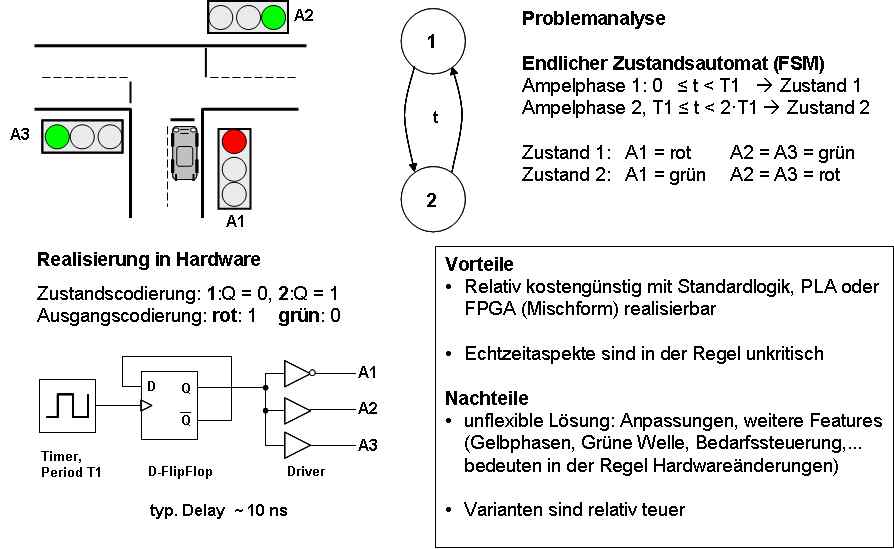
\includegraphics[width=14cm, height=9cm]{Images/image12.png}
    %\caption{Moore's Law}
    \label{fig:Fig 3}
\end{figure}

\begin{figure}[h]
    \centering
    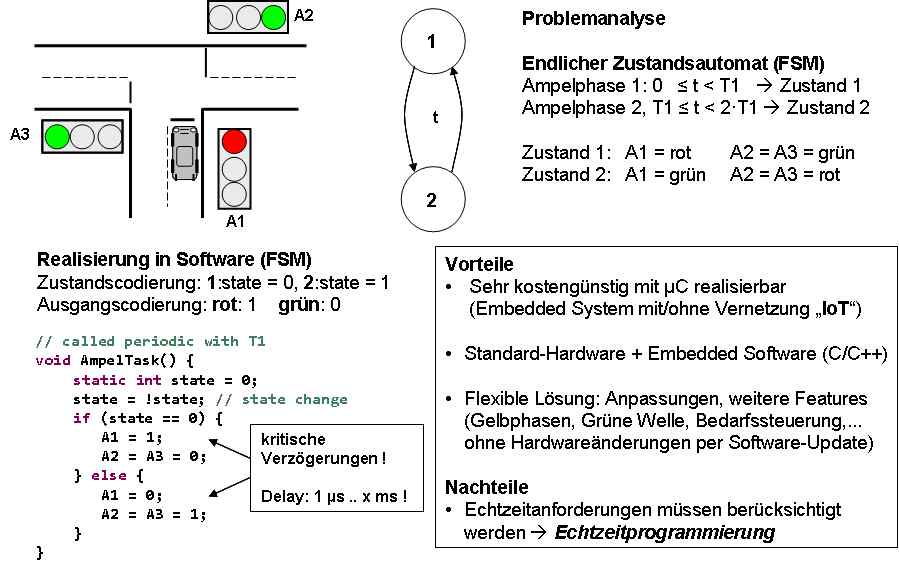
\includegraphics[width=14cm, height=8cm]{Images/image13.png}
    %\caption{Moore's Law}
    \label{fig:Fig 3}
\end{figure}

\begin{figure}[h]
    \centering
    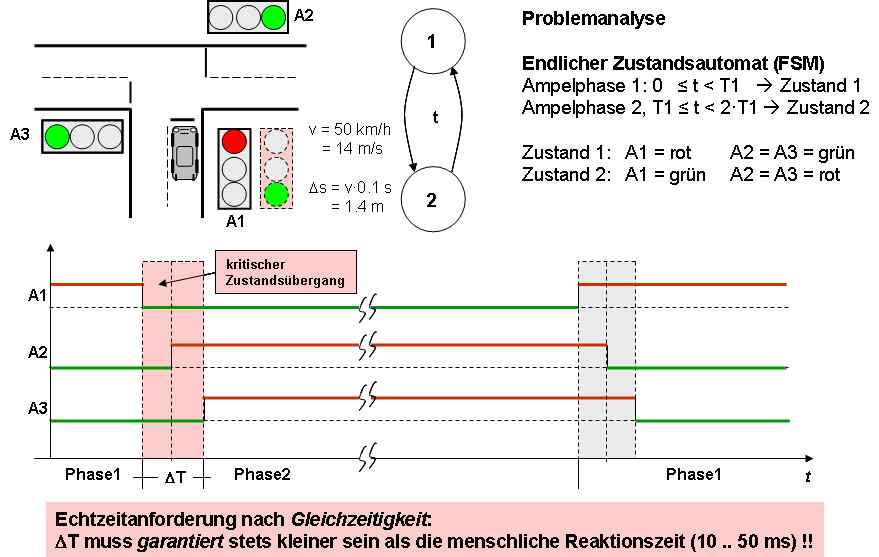
\includegraphics[width=14cm, height=8cm]{Images/image14.png}
    %\caption{Moore's Law}
    \label{fig:Fig 3}
\end{figure}

\newpage
\textbf{Solution}: Critical Section (Mutex) in AmpelTask:  see FSM Exercise

\begin{lstlisting}[style=mystyle, language=c]
 	// called periodic with T1  
	void AmpelTask() {
	static int state = 0;
	state = !state; // state change
  	begin(mutex);
	if (state == 0) {
		A1 = 1;
		A2 = A3 = 0;
	} else {
		A1 = 0;
		A2 = A3 = 1;
	}
  	end(mutex);
\end{lstlisting}

\newpage

{\rot\bf A Definition of Real-Time Systems is given by DIN 44300 [1985]}\\

\textit{ Realzeit-Systeme beziehungsweise Echtzeitsysteme sind Computersysteme, dieim Realzeitbetrieb arbeiten.}\\

\textit{Realzeitbetrieb wird definiert als der Betrieb eines Rechensystems, beidem Programme zur Verarbeitung anfallender Daten st\"{a}ndig betriebsbereitsind, derart, dass die Verarbeitungsergebnisse innerhalb einer vorgegebenenZeitspanne verf\"{u}gbar sind. Die Daten k\"{o}nnen je nach Anwendungsfall nacheiner zeitlich zuf\"{a}lligen Verteilung oder zu vorherbestimmten Zeitpunktenanfallen.}\\

{\rot\bf Wikipedia:}\\

In computer science, \textbf{real-time} computing (RTC), or reactive computing, is the study of hardware and software systems that are subject to a "real-time constraint", i.e., operational \textbf{deadlines} from \textbf{event to system response}. \\

By contrast, a \textbf{non-real-time system}  is one for which there is \textbf{no deadline}, even if fast response or high performance is desired or preferred. \\

The needs of real-time software are often addressed in the context of real-time operating systems, and synchronous programming languages, which provide frameworks on which to build real-time application software.\\

A real time system may be one where its application can be considered (within context) to be mission critical. \\

The anti-lock brakes on a car are a simple example of a real-time computing system - the real-time constraint in this system is the short time in which the brakes must be released to prevent the wheel from locking. \textbf{Real-time computations} can be said to have \textbf{failed if} they are \textbf{not completed before their deadline}, where their deadline is relative to an event. \\

\textbf{A real-time deadline must be met, regardless of system load}.\\

Thus, in a real-time system the logical correctness (functional correctness) of the answers with guaranteed response times (temporal correctness) is of essential importance. \\

The temporal behavior in real-time systems is part of the system specification and thus subject of the product verification.\\

\textbf{Embedded systems} often have to meet \textbf{real-time requirements}.\\

{\rot\bf Technical Process and Process Model}\\

A technical process can be defined as follows (DIN 66 201):\\

In a technical process materials, energy or information (the process media) are converted or transported (such as an end product) into grafted materials, energy or information. \\

Its input and state variables summarized in the vector \textbf{Z} can be measured with sensors and controlled by actuators: \\

\begin{figure}[h]
    \centering
    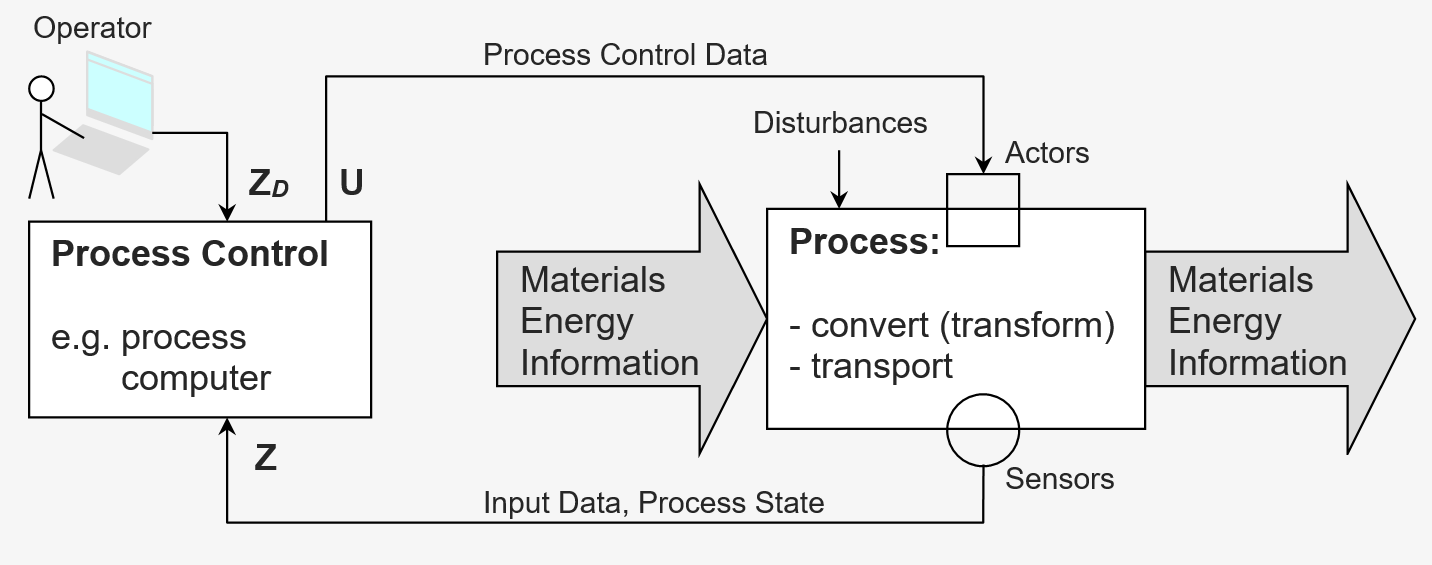
\includegraphics[width=14cm, height=6cm]{Images/image60.png}
    %\caption{Moore's Law}
    \label{fig:Fig 3}
\end{figure}

In automation, the process is controlled via control actions (vector \textbf{U}) so that after a given time, a desired process target or a desired state \textbf{Z\textit{${}_{D}$}} is reached. \\

The desired state can refer to the following:\\

quality, quantity (of the final product), speed, stability, security (during the transforming process), production, yield, raw material consumption, emissions, or even reaching the next process step (e.g. with sequential processes).\\

The delay time in the loop is of \textbf{\textit{crucial importance}} for the \textbf{\textit{stability}} of the \textbf{\textit{entire system}}!\\
This delay time must therefore be exactly specifiable  \textbf{\textit{Real-Time Programming}} !

\paragraph{  Timeliness}

The timeliness (=timing correctness) is directly derivable from the above considerations requirement for all real-time systems. For digital process computers timing correctness is, the output data must be calculated in time.

This also requires that the input data must be collected on time. The timing deadlines, and are usually given by a technical process:

Thus the allowed response time for the controller is limited to a known value, thus real-time systems are said to be \textbf{predictable} or \textbf{deterministic}.

Input data must be read in time for a real-time system, and the output data to be generated must be provided within the given deadline (time condition). 

The primary requirement for a real-time control is the \textbf{constant ability to input, process and output data on time regardless of the system workload}. 

For a real-time system also means that it \textbf{monitors the temporal validity} of information and prevents the use of invalid data !

This must apply regardless of whether the data to be processed are \textbf{event based} or at \textbf{predetermined (e.g. periodic) times}.

However, due to complexity, the timing behavior of real-time systems \textbf{can never be predicted with 100~\% certainty}  System validation by tests !

\paragraph{  Time Conditions}

The \textbf{time conditions} to monitor, and control a process can be in several variants

\begin{enumerate}
\item  Precise Time, Exact Time A precise time \textit{t}${}_{0}$ for a controller action is defined. This action must not be executed earlier or later. \textbf{Examples}: Sampling Systems (DSP \& Digital Control),      clock display control.

\item  Latest Time Limit, DeadlineA maximum time \textit{t}${}_{max}$ (=deadline) for a controller action is defined. This action must be finished latest at its deadline, but it can be finished earlier. \textbf{Examples}: a sampling system calculating an output sample for the next sampling      period, Anti-Squeeze Control, maximum response time with switching      on/off a machine, UI control reaction time to a button, slider, {\dots}      e.g. \textit{t${}_{max}$} $\mathrm{<}$ 50ms with human reaction times  ``\textit{immediately}''    

\item  Earliest Time Limit A minimum time \textit{t}${}_{min}$ for a controller action is defined. The action must not be executed earlier, but it can be executed later. \textbf{Examples}: transitions in state machines, an output may not occur before a state       transition has been finished.

\item  Time IntervalAn action must be executed within a time interval [\textit{t}${}_{min}$, \textit{t}${}_{max}$], thus at any time earlier than \textit{t}${}_{max}$ and later than\textit{ t}${}_{min}$. \textbf{Example}:  airbag ignition in some crash situations an airbag shall be ignited      e.g. 10-30 ms, in other situations 5-8 ms after crash.
\end{enumerate}

Time conditions can be \textbf{periodic} or \textbf{non-periodic}. 

\textbf{ Periodic Time Condition }

A periodic time condition is given with analog signals to be sampled and processed by a digital computer. Any analog signal has to be discretized in both value and time by a constant periodic sampling time \textit{T}${}_{s}$. This is typical for sampling systems realizing digital filters or digital control algorithms for processing quasi analog signals.

An example is the electric signal of a microphone which has to be sampled \textbf{strictly periodic} in order to have a \textbf{digital representation} of the \textbf{original analog sound signal}. Any deviation from the periodic sampling results in unwanted noise, which cannot be compensated. After time sampling the values of the voltage signal is discretized by an AD-Converter.

\textbf{Sampling Theorem [Kamm], [Oppen]}

\textbf{Example}: CD-Audio: \textit{f}${}_{s}$ = 44.1 kHz, \textit{T}${}_{s}$ = 22.7 µs  \textit{B${}_{x}$} = 20 kHz $\mathrm{<}$ 0.5 \textit{f}${}_{s}$ = 22.05 kHz 

Correct sampling:       tagesschau\_44.1.wav    Sampling theorem violation:  tagesschau\_D10.wav

Digital signal processing of analog signals involves very strict requirements to real-time conditions, due to the periodic and exact sampling conditions.

\begin{tabular}{|p{2.2in}|p{1.9in}|} \hline 
\textbf{Action} & \textbf{Time Condition} \\ \hline 
input of a sample of an analog signal    & exact periodic sampling at  k$\mathrm{\bullet}$\textit{T}${}_{s}$ \\ \hline 
computation of a signal sample  & time interval [k$\mathrm{\bullet}$\textit{T}${}_{s}$ + \textit{T${}_{ADC}$,} (k+1)$\mathrm{\bullet}$\textit{T}${}_{s}$] \\ \hline 
output of the calculated signal sample & exact periodic sampling at  (k+1)$\mathrm{\bullet}$\textit{T}${}_{s}$ \\ \hline 
\end{tabular}

\textbf{ Non-Periodic Time Condition}

A non-periodic time condition is given frequently with digital signals to be processed at arbitrary, non-predictable times due to events like pushing or releasing a switch or a revolution sensor, producing a slope at discrete angles of a motor shaft.

\textbf{Absolute Time Condition }With an absolute time condition defined, an action must be executed at a certain global time, i.e. an action must be performed at 12:00:00 MEZ.

\textbf{Relative Time Condition }With a relative time condition defined, an action must be executed relative to some previous event. Example: a control signal must be updated after 0.5~s after a push button was pressed.

All time conditions can arise in combinations.

For meeting the time conditions a real-time system must have

\begin{enumerate}
	\item  \textbf{sufficient processing speed} to process the input and output data at the required speed (sampling frequency), which the technical process requires
	\item  \textbf{deterministic time behavior}
\end{enumerate}

\paragraph{  Hard and Soft Real-Time Systems}

In the previous section, we saw that computation must complete before reaching a given deadline. In other words, real-time systems have timing constraints and are deadline-driven. Real-time systems can be classified, therefore, as either hard real-time systems or soft real-time systems.

What differentiates hard real-time systems and soft real-time systems are the degree of tolerance of missed deadlines, usefulness of computed results after missed deadlines, and severity of the penalty incurred for failing to meet deadlines.

For \textbf{hard real-time systems}, the level of tolerance for a missed deadline is extremely small or zero tolerance. The computed \textbf{results after} the \textbf{missed} \textbf{deadline} \textbf{are} likely \textbf{useless} for many of these systems. The penalty incurred for a missed deadline is \textbf{catastrophic} (e.g. an unstable control loop). 

For \textbf{soft real-time systems}, however, the level of tolerance is non-zero. The computed \textbf{results after} the \textbf{missed deadline} have a \textbf{rate of depreciation}. The \textbf{usefulness} of the results does \textbf{not reach zero immediately} passing the deadline, as in the case of many hard real-time systems. The physical impact of a missed deadline is\textbf{ non-catastrophic}.

\begin{enumerate}
	\item  \textbf{Hard Real-Time Conditions} the time conditions must be met, or catastrophes occur !  Deviations from the time-conditions are not allowed and represent a serious error. In safety-related systems a violation of the hard real-time time conditions can endanger human life (e.g. if sampling controls become unstable). Systems, meeting the hard real-time conditions are called \textbf{\textit{Hard Real-Time Systems}}. \textbf{Examples}: Sampling Controls (closed-loop), aerospace flight controls, airbag ignition, automotive X-by-wire, pacemakers, {\dots} 
	\item  \textbf{Soft Real-Time Conditions} the deadlines must be met but with a degree of flexibility. The deadlines can contain varying levels of tolerance, average timing deadlines, and even statistical distribution of response times with different degrees of acceptability. A missed deadline does not result in system failure, but costs can rise in proportion to the delay, depending on the application. Systems meeting soft real-time conditions are called \textbf{\textit{Soft Real-Time Systems}}.\textbf{Examples}: multimedia-streams (speech, video, music, low level audio), toasters, refrigerators, {\dots} 
\end{enumerate}

\paragraph{  Concurrency}

Real-time systems must generally treat multiple inputs and outputs simultaneously. Thus, the simultaneous addition to the timeliness of the second general requirement for real-time systems.

Example is about a CNC machine tool, where the x-y axes must be controlled simultaneously (synchronously, concurrently) to move the tool along a predetermined path \textit{B}(\textit{x}, \textit{y}) = \textit{B}(\textit{x}(\textit{t}), \textit{y}(\textit{t})). 

There is an relative time condition for both processes acting concurrently on the two drive axes x and y:

If the time axis of x and y are shifted by some amount of time $\Delta$\textit{T} (e.g. due to different clocks for x- and y-drive control), the resulting path \textit{B}(\textit{x}, \textit{y}) = \textit{B}(\textit{x}(\textit{t}), \textit{y}(\textit{t-}$\Delta$\textit{T})) will be wrong.

\textbf{Example}: Tolerances {\textbar}\textit{x}{\textbar}, {\textbar}\textit{y}{\textbar} $\mathrm{<}$ 0.05 mm,   Requirement    \textit{v${}_{x}$} = \textit{v${}_{y}$} = \textit{x}' = \textit{y}' = $\mathrm{\pm}$10 cm/s     Requirement     {\textbar}\textit{t}{\textbar} $\mathrm{<}$ {\textbar}\textit{x}{\textbar} / {\textbar}\textit{v${}_{x}$}{\textbar} = 0.5 ms       Synchronization, Real-Time Condition

\textbf{ Realizations of Real-Time Systems with Concurrency Requirement}

To meet the requirement of concurrency, there are several possibilities:

\begin{enumerate}
	\item  Full parallel processing in a multiprocessor system
	\item  Quasi-parallel processing in a multiprocessor system
	\item  Quasi-parallel processing in a uniprocessor system (\textbf{Multitasking})
\end{enumerate}

\begin{enumerate}
	\item  Each task is processed on a separate processor (e.g. microcontroller). There is a real parallel processing, each task has the full power of its own processor. This allows the independent consideration of each task, however, the tasks must be synchronized in most cases (e.g. x-y axis control of the CNC machine).
	\item  Each task executed on a processor that is allocated by a real-time scheduler(there are usually fewer processors available than tasks). The real-time scheduler is a hardware or software component, which assigns the tasks to processors such that all tasks can meet their timing constraints.The individual tasks can be assigned to single processors.
	\item  From a hardware perspective, the simplest and most cost effective and realization: All tasks share a single processor Multitasking. A Real Time Scheduler controls the allocation of the processor to the task. This form of real-time scheduling is the easiest to analyze and control  preferred realization of most embedded systems.
\end{enumerate}

\paragraph{  Availability}

Real-time systems must be available without interruption, otherwise time conditions may be violated. This leads to the third basic requirement of real-time systems, the \textbf{availability}. 

Real-time systems must be available over a longer period of time, maybe around the clock without any breaks, as with

\begin{enumerate}
	\item  Power Plant Controls
	\item  Production Facilities
	\item  Heating and Air Conditioning Systems
	\item  Communication
	\item  Medical Applications 
	\item  ...
\end{enumerate}

This requires that there is no disruption of operations for phases of system reorganization. A typical example here is the garbage collection of some programming languages such as Java or C \# or their runtime environments. For example, the default Java implementation is not suitable for use in real-time systems. Remedy is the use of algorithms free of need for reorganization (such as for dynamic memory management).

\textbf{Example}: Algorithm for Calculation of a Factorial in C OK with Real-Time programming      Not OK with Real-Time programming ! (Exec.-Time of stack operations not deterministic due to recursion). Another possibility is to divide the reorganization into small steps under control of the real-time scheduler to ensure that no time constraint is violated: This method is been used by Real-Time Java (Real-Time Specification for Java (RTSJ)).Also, more traditional memory management strategies involve not predictable time for execution (like \textbf{malloc/free} of the C standard library, \textbf{new/delete} with C++)  dynamic memory management is typically avoided with hard real-time systems !

\textbf{Example}:

Not OK with Real-Time programming     OK with Real-Time programming !(Exec.-Time of malloc() non deterministic)

- but: malloc() in initialization possible  

\subsection{  Timing Definitions}

\textbf{Process Time and Processing Time}

The time interval between two requests of the same type is called the \textbf{process time} \textit{T${}_{P}$}. If the interval between two events is constant, it is called a periodic event. 

In many cases, however, the time interval varies, so that there is a time interval with a minimum \textit{T${}_{Pmin}$} and a maximum \textit{T${}_{Pmax}$}.

For the actual processing of the event computer instructions (operations) have to be executed. The event belongs to the sequence of instructions is referred to as the code sequence or a job. Jobs are implemented within the computer as a computational process, which can be distinguished as \textbf{tasks} and \textbf{threads} (see section \textbf{Process Management}). 

For the execution of a job i the computer needs \textbf{processing time} \textit{T${}_{Vi}$} (from de: \textit{Verarbeitungszeit}) which is also called \textbf{execution time}.

The \textbf{processing/execution time }needed for a certain number of operations \textit{N} is inverse to the \textbf{computing power} \textbf{\textit{P}} (in ops / sec) a processor core (CPU) offers:

\begin{tabular}{|p{0.3in}|p{3.9in}|p{0.4in}|} \hline 
 & \textit{T${}_{V}$} = \textit{N} / \textit{P    }[\textit{T${}_{V}$}] = ops / (ops / sec) = sec\newline  & (1.1)
\end{tabular}

The CPU power is approximately proportional to the CPU clock frequency.

In practice it is not easy to specify the processing/execution time for a certain task, since it often depends on the input values (conditional branches). Furthermore, the performance of the processor varies (due to caches, pipelines and DMA). To calculate \textit{T${}_{Vmax}$} in real-time systems, \textit{N${}_{max}$} and \textit{P${}_{min}$} shall be used in \eqref{GrindEQ__1_1_}.

\textbf{Timeliness, Response time and Maximum Response Time}

Timeliness means, that a task required at the time \textit{t}${}_{0}$

\begin{enumerate}
	\item  is done \textbf{not before} a specified time \textit{t}${}_{0}$ + \textit{T${}_{Zmin}$} and
	\item  is done \textbf{no later} than a specified time \textit{t}${}_{0}$ + \textit{T${}_{Zmax}$} (timeliness).
\end{enumerate}

The requirement for a minimum latency, i.e, that a task is not been done before a certain time, is often missing (\textit{T${}_{Zmin}$} = 0) or can be realized easily. On the other hand, the requirement for \textbf{timeliness} (\textit{T${}_{R\ }$}$\mathrm{<}$ \textit{T${}_{Zmax}$}) is hard to guarantee. The \textbf{maximum reaction time} \textit{T${}_{Rmax}$} is the worst-case time when task execution ends and the computer can cause a reaction. The \textbf{maximum reaction time} \textit{T${}_{Rmax}$} always needs to be \textbf{smaller} than the \textbf{maximum response time} \textit{T${}_{Zmax}$}.

\textbf{Utilization, Load}

The computer core (CPU, processor) is loaded (utilized) depending on the frequency of occurrence of an event. The utilization  gives a relative measure how much the CPU is loaded by a task is the quotient of the necessary processing time \textit{T${}_{V}$} and process time \textit{T${}_{P}$}

\begin{tabular}{|p{0.3in}|p{3.9in}|p{0.4in}|} \hline 
 &  = \textit{T}${}_{V\ }$/ \textit{T}${}_{P}$ & (1.2) \\ \hline 
\end{tabular}

The total utilization ${}_{ges}$ is the sum of the utilization of all individual jobs \eqref{GrindEQ__1_3_}. A real-time system must be able to process all tasks with fulfilling their requirements for timeliness -- this is sometimes referred to as the requirement for concurrency (in a wider sense). Mathematically, this means that the total utilization \textit{${}_{ges}$} is less than 100\%:

\begin{tabular}{|p{0.3in}|p{3.9in}|p{0.4in}|} \hline 
 & $\begin{array}{l} {\rho _{ges} =\sum _{i=1}^{n}\rho _{i} = \sum _{i=1}^{n}\frac{T_{Vi} }{T_{Pi} }  } \\ {\rho _{ges} <\, \, 1} \end{array}$ & (1.3) \\ \hline 
\end{tabular}

\subsection{  Real-Time Evidence}

Evidence that all time requirements of all requests are met under all conditions, is very difficult (practically impossible). In principle, the real-time evidence is based on

\begin{enumerate}
	\item  evaluate the relevant characteristics of the technical process,
	\item  number of different requirements
	\item  Minimum processing time for each request
	\item  Minimum allowable response time for each request \textit{T${}_{Zmin}$}
	\item  Maximum allowable response time for each request \textit{T${}_{Zmax}$}
	\item  dependencies between events
	\item  identify the maximum processing time \textit{T${}_{VMax}$} (WCET = Worst Case Execution Time) for each request
	\item  check the\textbf{ load condition} \eqref{GrindEQ__1_3_}
	\item  verify the \textbf{timeliness condition} (determination of \textit{T${}_{Rmin}$} and \textit{T${}_{Rmax}$}).
\end{enumerate}

With verifying the \textbf{timeliness condition} in particular, it is not trivial to determine the maximum response time \textit{T${}_{Rmax}$}.

\textbf{ Estimate for the Worst Case Execution Time (WCET)}

The maximum processing time \textit{T${}_{VMax}$} -- often called Worst Case Execution Time (WCET) -- of a request is very difficult to determine. The WCET depends in particular on the algorithm, the implementation of the algorithm, the hardware used and the other activities of the system (other computing processes). Therefore, the WCET at best be estimated. In principle, two methods for determining the WCET can be distinguished:

\begin{enumerate}
	\item  measure the WCET 
	\item  static code analysis with WCET determination (count operations,cycle).
\end{enumerate}

\textbf{WCET Measure}

The WCET is determined by execution of the code sequence that will be processed, normally on the target platform. The time between the onset of the event and output at the end of the code sequence is determined. Condition: Modification of the real-time software

\textbf{Method for Measuring WCET}

To measure this time can be divided into two basic methods:

\begin{enumerate}
	\item  1st Measurement by the measure out piece of code itself (see above).The piece of code will be amended such that every time an event arrives and when the reaction took place, a time stamp\textit{ t}${}_{1}$ ( free running timer) is stored. At the end of the code, a second time stamp\textit{ t}${}_{2}$ is stored. the difference \textit{T${}_{Vi}$} = \textit{t}${}_{2}$ - \textit{t}${}_{1}$ is the actual execution timeThe first value \textit{T${}_{V}$}${}_{1}$ is stored as \textit{T${}_{Vmax}$}. With subsequent iterations, a newly calculated time \textit{T${}_{Vi}$}  is compared with the stored value. If the newly calculated time is greater than the previously measured WCET, the new value overwrites the existing WCET\textit{T${}_{Vmax}$} = max(\textit{T${}_{Vi}$})
	\item   External measurement of event and response (output), by means of an oscilloscope using port-toggle.
\end{enumerate}

For a WCET measure, appropriate input values and events must are generated. In addition, the entire system must be put under load (e.g. by an automatic tester).

\textbf{Advantages} of the method:

\begin{enumerate}
	\item  Independent of a programming language
	\item  Relatively easy to implement
	\item  Can run as autonomous self-diagnosis
\end{enumerate}

\textbf{Disadvantages} of the method:

\begin{enumerate}
	\item  The WCET of a code sequence can not be guaranteed, after all, it depends on many factors (background, loop iterations, caches, branches, etc ..).
	\item  The measurement is WCET is time consuming and ultimately expensive. Measure out the piece of code needs to be theoretically charged with all input data (in any combination).
	\item  This method can be carried out with the running code on the target platform only. Thus, an assessment at an early stage of development can be difficult.
	\item  A test environment is required (which provides the input data to create).
	\item  The code sequence to be measured out must be modified (for storing time stamps)  timers.
	\item  It is sometimes difficult to put the system under the required load.
\end{enumerate}

\textbf{ Static Code Analysis}

Here, the code itself is analyzed. Therefore most often an analysis tool program is used, which is fed with the object (machine) code, rather than with the C-source code. In addition, a hardware description is necessary (e.g. clock frequency of the microcontroller). 

The tool allows the duration of each code sequences to be estimated. After that, the number of loop iterations are considered, a bound of the number of cycles and the estimated execution time \textit{T${}_{SA}$} is printed.

Analysis can get rather complex, if cache hits, cache misses, processor pipelining are conssidered. 

If there are safety requirements, the code measured is not to changed after a static code analysis.

As a safety margin factors of \textit{c} = 2, 3, sometimes are used to state an upper limit

\textit{t}${}_{Vmax}$ $\mathrm{\le}$ \textit{T${}_{SA}$ }· \textit{c}

A manual determination of the number of cycles can be done in simple cases by inspection of the C-compiler generated assembler code:

Example: timer-interrupt routine for AVR microcontroller (e.g. ATmega8\_sum.pdf). The C-compiler generated assembly-/machine-code, ultimately determines the number of cycles to complete a section of code for a particular microcontroller (AVR here). The number of cycles multiplied by the instruction cycle time is the execution time.

\textbf{Estimation of the Best Case Execution Time (BCET)}

The determination Best Case Execution Time of a job can be done as the WCET, with the least possible load on the system, which can be easily implemented in general-at least in a test environment.

\textit{T${}_{Vmin}$} = min(\textit{T${}_{Vi}$})

\section{   Real-Time Operating Systems}

An \textbf{RTOS} (Real-time Operating System) must meet the same requirements as a standard general purpose operating system (GPOS) and offers services for


\begin{enumerate}
	\item  \textbf{Task Management}This is the management and organization of the implemented programs to be processed, also called tasks. The mission of the task management is thus essentially in the allocation of the processor (or the processors in a multiprocessor system) to the task.
	\item  \textbf{Resource Management}Tasks need resources for their execution, their allocation is the task of resource management. This mainly includes:- Memory management, responsible for allocating memory- Input/Output (I/O) management responsible for the allocation of I/O devices to  the tasks.
	\item  \textbf{Communication}The communication between tasks, called inter-process communication.
	\item  \textbf{Synchronization}A special form of communication is the synchronization, which refers to the timing of the tasks.
	\item  \textbf{Protection}The protection of resources against unauthorized access by tasks.
\end{enumerate}

These traditional requirements are exactly the same RTOSes as with GPOSes. Depending on the application, some of the services might be implemented only  rudimentary or completely absent. This is in particular with \textbf{embedded} \textbf{systems}, where the \textbf{RTOS} is kept as \textbf{lean as possible}, due to the limited resources.

In addition to the traditional OS requirements, real-time operating systems are required to 

\begin{enumerate}
	\item  Respect for timeliness and concurrency,
\end{enumerate}

\begin{enumerate}
	\item  Respect for availability.
\end{enumerate}

These requirements of RTOS dominate the other requirements, even if compromises are necessary.

\subsection{  Structure of an RTOS}

A real-time operating system (RTOS) is a program that schedules execution in a timely manner, manages system resources, and provides a consistent foundation for developing application code. Early operating systems had a monolithic structure, i.e. all functionality was implemented in a uniform, not further subdivided software block. This led to a number of disadvantages such as poor maintainability, poor adaptability and high error rate. Today's operating systems therefore follow a hierarchical layers model. 

\begin{enumerate}
	\item  \textbf{Device Driver}: This layer abstracts from the hardware, and- realizes the \textbf{hardware-dependent} \textbf{control} of each device - realizes the \textbf{hardware-independent} interface for the above layer. Ideally, the device drivers are the only hardware dependent layer in the OS. When adapting to other devices, only the device driver layer must be changed.
	\item  \textbf{I/O (Input-/Output) Control}, realizes the \textbf{logical}, \textbf{hardware-independent} device control. 
	\item  \textbf{Resource Management}: responsible for (allocation) and de-allocation (release) of memory and I/O resources.
	\item  \textbf{Task Management}: responsible for the allocation of the processor to each task. 
	\item  \textbf{API (Application Program Interface)} realizes the interface to the application.
\end{enumerate}

The OS kernel is critical for the stability and security, it is executed in the so-called \textbf{\textit{kernel mode}} of the processor, which allows full access to all resources.

The \textbf{\textit{kernel mode}} is a special operating mode of (advanced) microprocessors, enabling privileged instructions, direct access to memory and I/O, change configuration registers, etc.

In normal \textbf{\textit{user mode}} this privileged commands are blocked so that an application can not interfere with important operating system parts. This is one of the protection services of the operating system.

In the previous layer model, the core operating system extends over the layers 1 -- 4. Since the core contains many layers, it is called a \textbf{macro core operating system}.

Today's RTOSes must be highly configurable, especially in the field of \textbf{embedded systems} where scarce resources are typical  FreeRTOS.

It is therefore desirable to remove unwanted parts from the operating system, e.g. not needed scheduling or protection methods. This leads to the concept of the \textbf{micro-kernel operating system}.

\subsection{ Task Management}

The task management is a core task of operating systems. The most significant differences between standard and real-time operating systems are found here.

The tasks in a real-time application must meet the requirements for timeliness and concurrency. This requires scheduling strategies for RTOSes different from those found in  standard operating systems.

\paragraph{  Task Model}

A \textbf{computational process} or \textbf{process} (also called \textbf{task}) is running as a computer program together with all the variables (including register states) and resources each process has a \textbf{main()}

A task is a process controlled by the RTOS for execution of a sequential program. Several tasks are being processed by the quasi-parallel processor, necessary changes between tasks are made by the RTOS' task scheduler.

Changes between tasks are needed to meet all tasks requirements for timeliness.

Within a \textbf{\textit{process}}, there can be parallel \textbf{\textit{threads}} (running simultaneously). 

A \textbf{\textit{thread}} must share its resources with other \textbf{\textit{threads}} of the same \textbf{\textit{process}}  just${}_{\ }$1${}_{\ }$\textbf{main()}

\begin{enumerate}
	\item  A \textbf{task} is called a \textbf{heavyweight process, }if it contains its own variables and resources separated from other tasks by the OS. It has its own address space and can communicate with other tasks via interprocess communication. A task realized as a process provides maximum protection, possible interference by other tasks is limited to predefined channels. A change of the processor to another task (\textbf{context switch}) is due to the separate resources, which is a time-consuming task.
	\item  A \textbf{task} realized as a \textbf{thread} is called a \textbf{lightweight process} that exists within a single process. It uses the variables and resources of the process. All threads within a process \textbf{share the same address space}. Communication can take place over any global variable within the process. Threads can interfere with any other thread within a task.  Shared memory allows great efficiency. Communication between threads is more direct and faster Context switch can take place very quickly, e.g.: FreeRTOS, VxWorks Low data protection between data of individual threads
\end{enumerate}

To fulfill the \textbf{real-time requirements}, efficiency is usually more important than protection. 

Many real-time applications use \textbf{threads within a single task}.

Often, a real-time application is realized by a \textbf{\textit{single}} \textbf{\textit{process}}, which contains threads to realize numerous tasks.\textbf{ Embedded systems} are often based on the \textbf{thread concept}, due to scarce resources.

From the perspective of the real-time conditions (timeliness, concurrency, availability), \textbf{threads} aren't different from \textbf{processes}, both are usually identified by the term \textbf{task}.

\paragraph{ Multitasking, Context Switch }

Multitasking is the ability of the OS to handle multiple tasks within set deadlines. An RTOS kernel might have 2 tasks that it has to schedule to run. At certain times, execution of Task 1 has to switch to Task 2

\paragraph{  Task States}

For each task (or threads) one can define 6 different states:

\begin{enumerate}
	\item  \textbf{existent}
	\item \textbf{ ready (}waiting\textbf{)}The task is ready, all conditions are fulfilled, resources are allocated, the task is waiting for the allocation of the processor.
	\item  \textbf{running }(executing)The task is run on the processor. In a uniprocessor only one task can be in this condition, in a multi-processor system, several tasks can be in this state simultaneously. 
	\item  \textbf{blocked} (blocked)The task is waiting for an event (e.g. an input value, an inter-process communication object) or the release of a resource (task synchronization). 
	\item  \textbf{suspended }(finished)A task is suspended from its normal operations by another task. It can be resumed later
	\item  \textbf{not existent}
\end{enumerate}

\subsection{  Real-Time Scheduling}

The main job of an RTOS task management is the allocation of the processor to the ready tasks. There are different strategies, so-called scheduling strategies.

A \textbf{real-time scheduler} must divide all ready (runnable) tasks to the processor, so that all all time conditions are met. The set of tasks managed by the real-time scheduler is called \textbf{taskset}.

For the evaluation of various scheduling strategies, the processor demand \textit{H} (=\textbf{utilization}) is an important quantity for the load of the processor, it is defined as

\begin{tabular}{|p{0.3in}|p{3.9in}|p{0.4in}|} \hline 
 & \textit{\newline H} =\newline  & (2.1) \\ \hline 
\end{tabular}

Each CPU can be utilized up to 100 \% at maximum.\textbf{  Example}: A periodic task 1 with a period of \textit{T}${}_{P1}$ = 200 ms and an execution time of \textit{T}${}_{e1}$ = 100 ms causes a processor demand of \textit{H}${}_{1}$ = 50 \%

A second periodic task with a period of \textit{T}${}_{P2}$ = 100 ms and an execution time of \textit{T}${}_{e2}$ = 50 ms also causes a processor demand of \textit{H}${}_{2}$ = 50 \%. 

An implicit timing condition for each periodic task is: task execution must be finished before the next period starts (deadline) !

Both tasks cause a total processor demand \textit{H} = \textit{H}${}_{1}$ + \textit{H}${}_{2}$ = 100~\%.

One possible schedule for executing both tasks is to displace task 1 after exactly half of its execution time by task 2, which is never displaced. Thus, task 1 must be displaceable:

another possible schedule:

In general, for a tasklet of \textit{n} periodic tasks, the total processor demand

\begin{tabular}{|p{0.3in}|p{3.9in}|p{0.4in}|} \hline 
 &         $H=\sum _{i=1}^{n}\frac{T_{ei} }{T_{pi} }  $ & (2.2) \\ \hline 
\end{tabular}

\paragraph{  Classification of Scheduling Algorithms}

\textbf{Static Scheduling}

Prior to the execution of a taskset an allocation table (dispatching table) with the start times exists, regarding time constraints and dependencies of each task. The dispatcher as part of the RTOS kernel assigns the individual tasks due to this table 

 principle of synchronous programming.

Advantage  minimal overhead, as no decisions are needed at runtime. 

Disadvantage  restriction to periodic events.

\textbf{Dynamic Scheduling}

Here for the execution of tasks different criteria are used by the dispatcher \textbf{at runtime}, taking into account start times, time conditions (deadlines), and dependencies of each task. Asynchronous programming. Advantage  increased flexibility and the opportunity to respond to aperiodic events. Disadvantage  increased overhead, lower predictability

\textbf{Static and Dynamic Priorities}

(Not to be confused with static/dynamic scheduling). The scheduler can use priorities for the allocation of resources (processor, memory, I/O,{\dots}) to a task. \textbf{Static priorities} are set before running the application and are never changed during runtime. \textbf{Dynamic priorities} can be adjusted for each task \textbf{at runtime}. Furthermore, there are algorithms, using \textbf{No Priorities} at all. 

\paragraph{ Preemption}

(= "Prioritization") is an important feature for a scheduler, which describes the capability for displacing a running task for later execution in favor of another task. 

\textbf{Preemptive scheduling }means that a less important task can be displaced by a more important task. The most important task with \textbf{\textit{ready}}-state will be executed immediately. The less important task will be continued again until no other more important task waits with \textbf{\textit{ready}}-state.

\textbf{(a) Preemptive Scheduling          (b) Non-Preemptive Scheduling }

\textbf{Non-preemptive scheduling} (= \textbf{cooperative scheduling}) means, that there is no displacement of a running task. Only after the current task is finished or blocked, the next task with \textbf{\textit{ready}} state is executed.


\paragraph{  Time-Slice Scheduling (Round-Robin Scheduling)}

Time-Slice Scheduling (time slicing) assigns each task a fixed time slice (Time Slice). The order of task execution corresponds to the sequence of \textbf{\textit{ready}}-tasks entering the task-list of the OS scheduler (FIFO principle). The duration of the time slice for a task can be set individually.


This type of time-slice scheduling is a dynamic preemptive scheduling. 

 TSS does not use priorities

 time slot duration can be chosen individually for each task

 With time slices chosen fine-grained enough TSS is approaching optimality.

\textbf{Principle of Time-Slice (Round-Robin) Scheduling: }

\begin{enumerate}
	\item  All \textbf{\textit{ready}}-tasks are queued in a FIFO 
	\item  Each task \textit{i} gets assigned a time slice (time slice, quantum) \textit{T${}_{TSi}$}
	\item  If a task after the expiry of its quantum is still \textbf{\textit{running}},
	\begin{enumerate}
		\item  the task is preempted, i.e. displaced to the \textbf{\textit{ready}} state
		\item  the task is put at the end of the FIFO queue;
		\item  The first task in the FIFO will be executed.
	\end{enumerate}
	\item  If a task changes state from \textbf{\textit{blocked}} to \textbf{\textit{ready}}, it will be put at the end ofthe FIFO queue
\end{enumerate}

Typical Applications: \textbf{Kernel-mode programs  Example 1:} 3 Tasks with \textit{H}${}_{max}$ $\mathrm{<}$ 0.778, from [W\"{o}rnB] , same as in section 2.2.7: Task T1: period \textit{T}${}_{p1}$ = 10~ms, execution time \textit{T}${}_{e1}$ = 1~ms  \textit{H}${}_{1}$ = 0.1Task T2: period \textit{T}${}_{p2}$ = 10~ms, execution time\textit{ T}${}_{e2}$ = 5~ms  \textit{H}${}_{2}$ = 0.5Task T3: non-periodic, period \textit{T}${}_{p3}$ = deadline \textit{T}${}_{d3}$ = 15.4~ms, \textit{T}${}_{e3}$ = 2.62~ms  \textit{H}${}_{3}$ = 0.17

By \eqref{GrindEQ__2_2_} the total CPU utilization \textit{H} = 0.1 + 0.5 + 0.17 = 0.77 

One chooses a basic time-slice \textit{T}${}_{TS}$ = 1 ms and assigns individual time slices as multiples of \textit{T}${}_{TS}$ with $\Sigma$\textit{T}${}_{TS}$ = 9~ms:

Task T1:    \textit{T}${}_{TS1}$ = 1 $.$\textit{T}${}_{TS}$ = 1 ms  \textit{H}${}_{1}$ = \textit{T}${}_{TS1}$/$\Sigma$\textit{T}${}_{TS}$ = 1~ms / 9~ms = 11~\%

Task T2:    \textit{T}${}_{TS2}$ = 5 $.$\textit{T}${}_{TS}$ = 5 ms  \textit{H}${}_{2}$ = \textit{T}${}_{TS2}$/$\Sigma$\textit{T}${}_{TS}$ = 5~ms / 9~ms = 55~\%

Task T3:     \textit{T}${}_{TS3}$ = 3 $.$\textit{T}${}_{TS}$ = 3 ms  \textit{H}${}_{3}$ = \textit{T}${}_{TS3}$/$\Sigma$\textit{T}${}_{TS}$ = 3~ms / 9~ms = 33~\%

(a)

In this example the assigned time slices were chosen to be larger than the execution times of each task, in order to avoid preemption.

With TSS a context-switch can occur at the end of a time-slice only. which can cause some \textit{jitter} (as with task T1 above).

\paragraph{ Fixed Time-Slice-Scheduling }

FT scheduling is based on a TDMA approach, requires no priorities, and is therefore frequently used in embedded microcontroller applications without an operating system.

A strictly periodic schedule is created with a periodic time \textit{N·T${}_{TS}$}, i.e. with \textit{N} integer multiples of the basic \textit{T${}_{TS}$} time slice. Each task gets assigned one (ore more) basic time slots, large enough to hold the WCET of each:

Conditions for Events are polled within each task, if a task is not finished at the end of its timeslice, it can be preempted (\textbf{\textit{preemptive FTS}})or not (\textbf{\textit{cooperative FTS}}).

The previous example with three tasks, and an idle task T4 at a period \textit{N}$\mathrm{\bullet}$\textit{T${}_{TS}$} = $\Sigma$\textit{T${}_{TS}$} = 10 ms is realized, the time slices are chosen as multiples of \textit{T${}_{TS}$} = 1 ms as follows 

Task T1:    \textit{T${}_{TS}$}${}_{1}$ = 1 $.$\textit{T${}_{TS}$} = 1 ms  \textit{H}${}_{1}$ = \textit{T${}_{TS}$}${}_{1}$/$\Sigma$\textit{T${}_{TS}$} = 1~ms / 10~ms = 10~\%

Task T2:    \textit{T${}_{TS}$}${}_{2}$ = 5 $.$\textit{T${}_{TS}$} = 5 ms  \textit{H}${}_{2}$ = \textit{T${}_{TS}$}${}_{2}$/$\Sigma$\textit{T${}_{TS}$} = 5~ms / 10~ms = 50~\%

Task T3:     \textit{T${}_{TS}$}${}_{3}$ = 3 $.$\textit{T${}_{TS}$} = 3 ms  \textit{H}${}_{3}$ = \textit{T${}_{TS}$}${}_{3}$/2$\Sigma$\textit{T${}_{TS}$} = 3~ms / 10~ms = 30~\%

Task T4 (idle) \textit{T${}_{TS}$}${}_{4}$ = 1 $.$\textit{T${}_{TS}$} = 1 ms  \textit{H}${}_{4}$ = 10~\%

T3 runs for the second time at \textit{t} = 26 ms the delay of 10 ms does not result in a T3-deadline violation. The idle task T4 provides a placeholder for unused CPU load, which can be used in modern CPUs for power saving features.

\textbf{Advantage of fixed TSS}: the execution times can be defined exactly!

\paragraph{ Binary Fixed Time-Slice-Scheduling }

If task periodic times \textit{T${}_{Pi}$} can be represented as power-of-2 integer multiples of a basic time slice \textit{T${}_{TS}$}, one can obtain a periodic binary schedule:

If the maximum time of execution is \textit{T}${}_{TS}$ and equal for each task, the utilization for each task is 

\begin{tabular}{|p{0.3in}|p{3.9in}|p{0.4in}|} \hline 
 & $H_{i} =\frac{T_{ei} }{T_{pi} } =\frac{T_{TS} }{2^{i} \cdot T_{TS} } =2^{-i} $     $\sum _{i=1}^{N}H_{i} \stackrel{N\to \infty }{\longrightarrow}  \; 1$ & (2.3) \\ \hline 
\end{tabular}

Thus, the fastest task with periodic time \textit{T${}_{p}$}${}_{1}$ = 2$.$\textit{T}${}_{TS}$ is assigned 50~\% of the complete processing time, task 2 with periodic time \textit{T${}_{p}$}${}_{2}$ = 4$.$\textit{T}${}_{TS}$ gets assigned 25~\%, task 3 gets 12.5~\%, {\dots}

From \eqref{GrindEQ__2_3_} it shows, that the total utilization of \textit{H} aiming with an infinite number of tasks to 100\%, thus, there will be no overload situations, if all tasks meet their maximum execution time \textit{T${}_{TS}$} requirement (easily guaranteed with a preemptive schedule).

\textit{   T${}_{TS}$} $\mathrm{\ge}$ max(\textit{T${}_{e}$}${}_{1}$,\textit{ T${}_{e}$}${}_{2}$,\textit{ T${}_{e}$}${}_{3}$, ..)

With a non-preemptive schedule (cooperative task schedule) maximum execution times \textit{T${}_{ei}$} have to be determined carefully (WCET determination), such, that each task can complete execution within the basic \textit{T${}_{TS}$}. If a task gets delayed for some reasons (like high priority interrupts during execution) the complete schedule will get delayed.

\textbf{Advantages }

Binary fixed time-slice scheduling is

\begin{enumerate}
	\item  quite suitable with multirate sampling systems (e.g. oversampling, when integer multiples of a common sampling frequency are needed).
	\item  a very simple scheduling without priorities,
	\item  suitable in a non-preemptive realization for even small microcontrollers without OS. 
	\item  Time and duration of execution for each task is guaranteed (apart from interrupts)
\end{enumerate}

\textbf{Disadvantages }

\begin{enumerate}
	\item \textbf{ }Binary time-slice scheduling is not fully flexible with arbitrary periodic times and execution times
	\item  can turn into very complex software, especially with integrating tasks with execution time larger than \textit{T${}_{TS}$}.
\end{enumerate}



\textbf{Lab-Experiment}   \textbf{\underbar{AVR-Timer-Interrupts-(FTS-Scheduling)}}

\textbf{\underbar{Sketch for Arduino Nano}  (FixedTimeSlice.ino)}

\textbf{Example}: 4 periodic tasks (on an AVR µC, from section Digital PID Control with 4 Tasks) 

\textit{T${}_{p}$}${}_{1}$ = \textit{T${}_{p}$}${}_{2}$ = 1 ms, \textit{T${}_{p}$}${}_{3}$ = 16 ms, \textit{T${}_{p}$}${}_{4}$ = 8 ms

\textit{T${}_{e}$}${}_{1}$ = 50 µs, \textit{T${}_{e}$}${}_{2}$ = 0.3 ms, \textit{T${}_{p}$}${}_{3}$ = 40 µs, \textit{T${}_{p}$}${}_{4}$ = 40 µs

\textit{H}${}_{1}$ = 5 \%, \textit{H}${}_{2}$ = 30 \%, \textit{H}${}_{3}$ = 0.1/20 = 0.5 \%, \textit{H}${}_{4}$ = 0.05/20 = 0.25 \%  \textit{H} = 30.75 \%

Solution with Binary time-slice schedule with 3 Tasks, \textit{T${}_{TS}$} = 0.5 ms, \textit{T${}_{TS}$} $\mathrm{\ge}$ max(\textit{T${}_{ei}$}) = max(0.3, 0.05, 0.005 0.0025 ms) tasks with the same periodic times run in the same time-slice: T1 und T2 executed successively in the 2 Timeslice 2·\textit{T${}_{TS}$ }= 1 ms

\begin{tabular}{|p{0.2in}|p{0.2in}|p{0.1in}|p{0.1in}|p{0.1in}|p{0.1in}|} \hline 
\textbf{t/\textit{T${}_{Ts}$}} & \textbf{16} & \textbf{8} & \textbf{4} & \textbf{2} & \textbf{1} \\ \hline 
\textbf{0} & 0 & 0 & 0 & 0 & 0 \\ \hline 
\textbf{1} & 0 & 0 & 0 & 0 & 1 \\ \hline 
\textbf{2} & 0 & 0 & 0 & 1 & 0 \\ \hline 
\textbf{3} & 0 & 0 & 0 & 1 & 1 \\ \hline 
\textbf{4} & 0 & 0 & 1 & 0 & 0 \\ \hline 
\textbf{5} & 0 & 0 & 1 & 0 & 1 \\ \hline 
\textbf{6} & 0 & 0 & 1 & 1 & 0 \\ \hline 
\textbf{7} & 0 & 0 & 1 & 1 & 1 \\ \hline 
\textbf{8} & 0 & 1 & 0 & 0 & 0 \\ \hline 
\textbf{9} & 0 & 1 & 0 & 0 & 1 \\ \hline 
\textbf{10} & 0 & 1 & 0 & 1 & 0 \\ \hline 
\textbf{11} & 0 & 1 & 0 & 1 & 1 \\ \hline 
\textbf{12} & 0 & 1 & 1 & 0 & 0 \\ \hline 
\textbf{13} & 0 & 1 & 1 & 0 & 1 \\ \hline 
\textbf{14} & 0 & 1 & 1 & 1 & 0 \\ \hline 
\textbf{15} & 0 & 1 & 1 & 1 & 1 \\ \hline 
\textbf{16} & 1 & 0 & 0 & 0 & 0 \\ \hline 
\textbf{17} &  &  & 0 & 0 & 1 \\ \hline 
... &  &  &  &  &  \\ \hline 
\end{tabular}

\textbf{time-slice indexes}


\textbf{Proof for collision-free assignment of time-slice indexes } (with \textit{k},\textit{l} $\in$ \textbf{$\boldsymbol{\mathbb{Z}}$}  integers)

for some period \textit{N} we get time slices at indexes  \textit{n${}_{k}$}  =  \textit{k$\bullet$N  +  $\frac{N}{2} $}  e.g.: 2, 6, 10, 14, ..

thus, for period 2\textit{N} (next time slice) we get    \textit{m${}_{l}$} =  \textit{l$\bullet$}2\textit{N  +  N  }e.g.: 4, 12, 20, 28, ..

for a collision, we set \textit{n${}_{k}$} ${\mathop{=}\limits^{!}} $ \textit{m${}_{l}$}. Division by \textit{N} on both sides shows \textit{k} + 0.5 ${\mathop{=}\limits^{!}} $ 2$\mathrm{\bullet}$\textit{l} + 1, which has no solution with integers \textit{k} and \textit{l}, thus the above assignment is without any conflict all time slice indexes (proof by full induction) !


\paragraph{  FIFO Scheduling}

The name derives from the FIFO (first in, first out) principle of a waiting queue:    

\includegraphics*[width=3.78in, height=2.53in]{image16}

where elements put into a queue in a certain order of sequence, are taken out in the same order of sequence.With a \textbf{FIFO scheduler}, the tasks are processed in the same order in which they have taken the ready state.  An running task is not interrupted, it is a \textbf{non-preemptive}, \textbf{dynamic} scheduler.

Advantage:   very simple implementation, sometimes used in universal OS

Disadvantage:  bad real-time performance,        violations of time conditions even at low processing demands ( example)


\textbf{Example}: Two tasks with FIFO scheduling

Task 1: \textit{T}${}_{p1}$ = 150 ms, \textit{T}${}_{e1}$ = 15 ms   \textit{H}${}_{1}$ = 0.1

Task 2: \textit{T}${}_{p2}$ = 10 ms,  \textit{T}${}_{e2}$ = 1 ms    \textit{H}${}_{2}$ = 0.1

For both periodic tasks there is a time bound (deadline) with the next period. With \eqref{GrindEQ__2_2_}   \textit{H} = \textit{H}${}_{1}$ + \textit{H}${}_{2}$ = 0.1 + 0.1 = 0.2 

For 20~\% processor demand only, it should be easy to find a schedule for this taskset, but:

This simple example shows that even at a very low processor demand, a FIFO scheduler \textbf{cannot} \textbf{guarantee} compliance with the real-time conditions.


\paragraph{ Fixed-Priority Scheduling}

For fixed-priority scheduling, each task is assigned a fixed priority. The \textbf{\textit{ready}}-task with the highest priority waiting in the scheduler's queue is assigned to the processor.  fixed-priority scheduling is\textbf{ dynamic scheduling with static priorities}. (often used with interrupt processing of microprocessors, preemptive or non-preemptive):

\begin{enumerate}
	\item  \textbf{Fixed-Priority-Preemptive Scheduling (FPP)}If a \textbf{task with higher priority} than the currently running gets into the ready state, then the \textbf{current task is interrupted (displaced, preemted)} and the task with the higher priority is assigned to the processor immediately.
\end{enumerate}

\begin{enumerate}
	\item  \textbf{Fixed-Priority-Non-Preemptive Scheduling (FPN)}If a \textbf{task with higher priority} than the currently running gets into the ready state, then the \textbf{task is assigned} to the processor only \textbf{after the current task} is either \textbf{completed} or \textbf{blocked}.
\end{enumerate}


\textbf{Advantage}: with FPP, the compliance with the real-time conditions can be guaranteed (unlike to FIFO scheduling), if the priorities were assigned appropriate. 

The assignment of priorities to tasks is an important step in the development of a real-time application.

\textbf{Rate-Monotonic-Scheduling (RMS)}

For purely periodic applications, there is a rule, the so-called \textbf{rate-monotonic scheduling rule}, which states, that the priority of the tasks to be performed is inversely proportional to their periodic time:

\begin{tabular}{|p{0.3in}|p{3.9in}|p{0.4in}|} \hline 
 &       $PR_{i} \sim \frac{1}{T_{pi} } $ & (2.4) \\ \hline 
\end{tabular}

under the (rather idealized) conditions:


\begin{enumerate}
	\item  Preemptive scheduling is used
	\item  The periodic times \textit{T${}_{Pi}$} are constant 		
	\item  The time limits (deadlines) are equal to the periodic times \textit{T${}_{Pi}$}
	\item  The execution times are known and constant \textit{T${}_{ei}$}
	\item  The tasks are independent from each other (can not deadlock)
\end{enumerate}

\textbf{Example}: (same as with FIFO scheduling in section 2.2.6). Two tasks with Fixed-Priority-Preemptive Scheduling (FPP):

Task 1: \textit{T}${}_{p1}$ = 150 ms, \textit{T}${}_{e1}$ = 15 ms,   lower priority by   \eqref{GrindEQ__2_4_}

Task 2: \textit{T}${}_{p2}$ = 10 ms,  \textit{T}${}_{e2}$ = 1 ms   higher priority by \eqref{GrindEQ__2_4_}

The running task 1 is displaced with an event for task 2, which has higher priority (its state goes from \textbf{\textit{blocked}}  \textbf{\textit{ready}}), so that the deadline of task 2 is not violated (in contrast to FIFO scheduling).

Obviously,\textbf{ FPP scheduling} with \textbf{RMS} provides much better results than FIFO scheduling. 

In contrast, with \textbf{FPN}, the deadlines of task 2 would be violated !

In general

This also means that FPP scheduling with RMS always delivers an executable schedule, if one exists. However, the overall CPU utilization may not exceed \textit{H${}_{max}$ }([1], by Liu)

\begin{tabular}{|p{0.3in}|p{3.9in}|p{0.4in}|} \hline 
 &   $H_{\max } =n\cdot \left(2^{1/n} -1\right)=n\cdot \left(\sqrt[{n}]{2} -1\right)$ & (2.5) \\ \hline 
\end{tabular}

\begin{tabular}{|p{0.7in}|p{0.6in}|} \hline 
\textbf{\textit{n}} & \textbf{\textit{H${}_{max}$}} \\ \hline 
1 & 1.000000 \\ \hline 
2 & 0.828427 \\ \hline 
3 & 0.779763 \\ \hline 
4 & 0.756828 \\ \hline 
5 & 0.743492 \\ \hline 
10 & 0.717735 \\ \hline 
20 & 0.705298 \\ \hline 
50 & 0.697974 \\ \hline 
100 & 0.695555 \\ \hline 
1000 & 0.693387 \\ \hline 
10000 & 0.693171 \\ \hline 
\end{tabular}

The limit \eqref{GrindEQ__2_5_} can be used to examine the feasibility of a (periodic) taskset and to guarantee the conformance with all time limits.

FPP with RMS is very popular because of its simplicity. However, there are problems at very high utilization (beyond or near \textit{H${}_{max}$}) and with RMS at the same or nearly the same time periods, delivering same task priorities. Furthermore, there are sometimes difficulties in approaching non-periodic processes by periodic processes with sufficient precision.

\textbf{Example 1:} 3 Tasks with \textit{H}${}_{max}$ $\mathrm{>}$ 0.778, from [W\"{o}rnB] : Task T1: period \textit{T}${}_{p1}$ = 10~ms, execution time \textit{T}${}_{e1}$ = 1~ms  \textit{H}${}_{1}$ = 0.1Task T2: period \textit{T}${}_{p2}$ = 10~ms, execution time\textit{ T}${}_{e2}$ = 5~ms  \textit{H}${}_{2}$ = 0.5Task T3: non-periodic, deadline = \textit{T}${}_{d3}$ = 15.4~ms, execution time\textit{ T}${}_{e3}$ = 5.5~ms

By \eqref{GrindEQ__2_2_} the total CPU utilization \textit{H} = 0.1 + 0.5 + 0.357 = 0.957, amost 100 \% !But with \eqref{GrindEQ__2_5_} \textit{H} $\mathrm{>}$ \textit{H}${}_{max}$ $\mathrm{>}$ 0.78 deadlines will be violated with \textbf{FPP/RMS} with 3 tasks. 

FPP/RMS \textbf{can't deliver an executable schedule}, as this example shows:

By \eqref{GrindEQ__2_4_} one has 2 choices for assigning the priorities due to the equal periods \textit{T}${}_{p1}$\textit{ }and \textit{T}${}_{p2}$:

\textbf{Priority assignment (a)   Priority assignment (b)}

\begin{tabular}{|p{0.5in}|p{0.9in}|} \hline 
T1 & high priority \\ \hline 
T2 & medium priority \\ \hline 
T3 & low priority \\ \hline 
\end{tabular}

\begin{tabular}{|p{0.2in}|p{0.9in}|} \hline 
T2 & high  priority \\ \hline 
T1 & medium priority \\ \hline 
T3 & low priority \\ \hline 
\end{tabular}

In both cases there is a violation of the T3 deadline, if all tasks get \textbf{\textit{ready}} the same time at \textit{t} = 0: 

(a)


(b)


Of course, the violation of T3 deadline in the example above occurs due to the deliberate disregard of the load limit \textit{H${}_{max}$}, by \eqref{GrindEQ__2_5_}. If one meets the max. load requirement \textit{H} $\mathrm{<}$ 78\% (n = 3), there is violation of the T3 deadline.

However, with growing number of tasks the maximum load goes down as low as 70\% (from n $\mathrm{>}$ 10), which is surprisingly low.

Ideas to achieve higher processor loads lead to dynamic assignment of priorities.

 \textbf{Example 2:} 3 Tasks with \textit{H}${}_{max}$ $\mathrm{<}$ 0.778, from [W\"{o}rnB] : Task T1: period \textit{T}${}_{p1}$ = 10~ms, execution time \textit{T}${}_{e1}$ = 1~ms  \textit{H}${}_{1}$ = 0.1Task T2: period \textit{T}${}_{p2}$ = 10~ms, execution time\textit{ T}${}_{e2}$ = 5~ms  \textit{H}${}_{2}$ = 0.5Task T3: non-periodic, period \textit{T}${}_{p3}$ = deadline \textit{T}${}_{d3}$ = 15.4~ms, \textit{T}${}_{e3}$ = 2.62~ms  \textit{H}${}_{3}$ = 0.17

By \eqref{GrindEQ__2_2_} the total CPU utilization \textit{H} = 0.1 + 0.5 + 0.17 = 0.77 With \eqref{GrindEQ__2_5_} \textit{H} $\mathrm{<}$ \textit{H}${}_{max}$ = 0.78 deadlines will be not violated with FPP/RMS with 3 tasks:

By \eqref{GrindEQ__2_4_} one has 2 choices for assigning the priorities due to the equal periods \textit{T}${}_{p1}$\textit{ }and \textit{T}${}_{p2}$:

\textbf{Priority assignment (a)   Priority assignment (b)}

\begin{tabular}{|p{0.5in}|p{0.9in}|} \hline 
T1 & high priority \\ \hline 
T2 & medium priority \\ \hline 
T3 & low priority \\ \hline 
\end{tabular}

\begin{tabular}{|p{0.2in}|p{0.9in}|} \hline 
T2 & high  priority \\ \hline 
T1 & medium priority \\ \hline 
T3 & low priority \\ \hline 
\end{tabular}

In both cases there is no violation of the T3 deadline, even if all tasks get \textbf{\textit{ready}} the same time at \textit{t} = 0: 

(a)

(b)

If one meets the max. load requirement \textit{H} $\mathrm{<}$ 78\% (n = 3), there is violation of the T3 deadline.

However, with 3 tasks the maximum load allowed is as low as 77.8\% (for \textit{n} = 3), which is surprisingly low.

Ideas to achieve higher processor loads lead to dynamic assignment of priorities  next sections.

\paragraph{  Earliest-Deadline-First Scheduling (EDF)}

In Earliest-Deadline-First Scheduling (EDF) the Task Processor is granted to that \textbf{\textit{ready}}-task, which is closest to its time limit (deadline). This is achieved by assigning the task priorities according to the vicinity to the individual deadlines.

EDF is dynamic scheduling with dynamic priorities, either preemptive or non-preemptive

For \textbf{preemptive EDF scheduling} a context-switch is made, when a task with earlier time bound gets \textbf{\textit{ready}}. In \textbf{non-preemptive EDF scheduling} is the task with the shortest time interval ist executed only, if the currently running task is finished or blocked.

Preemptive EDF scheduling, is used more frequently than non-preemptive EDF scheduling, which is essentially only used when non-interruptible processes are to be managed, such as disk access.

\textbf{Advantage}: With \textbf{preemptive EDF scheduling }100 \% CPU utilization can be achieved. 

\textbf{Example} with 3 Tasks (same as in section 2.2.7): Task T1: period \textit{T}${}_{p1}$ = 10~ms, execution time \textit{T}${}_{e1}$ = 1~ms  \textit{H}${}_{1}$ = 0.1Task T2: period \textit{T}${}_{p2}$ = 10~ms, execution time\textit{ T}${}_{e2}$ = 5~ms  \textit{H}${}_{2}$ = 0.5Task T3: non-periodic, deadline = \textit{T}${}_{d3}$ = 15.4~ms, execution time\textit{ T}${}_{e3}$ = 5.5~ms(each periodic time is assumed to be deadline).

Again, by \eqref{GrindEQ__2_2_} the total CPU utilization \textit{H} = 0.1 + 0.5 + 0.357 = 0.957, almost 100 \% !

(at \textit{t} = 0, T1 and T2 have equal priorities, due to equal deadlines, in such a case, the scheduler decides randomly, e.g. for the task with the lower id)

It can be seen, that with EDF scheduling an executable schedule is found. 

Liu [W\"{o}rnB] shows, that EDF scheduling is an optimal scheduling with

\begin{tabular}{|p{0.3in}|p{3.9in}|p{0.4in}|} \hline 
 & \textit{ H} $\mathrm{<}$ 100~\%    for preemptive EDF scheduling & (2.6) \\ \hline 
\end{tabular}

\textbf{Advantage}: 

\begin{enumerate}
\item  as long as the processor utilization is less than 100 \% with a uniprocessor system, EDF  scheduling delivers an executable schedule and compliance with all time conditions is guaranteed.
\end{enumerate}

\textbf{Disadvantages:}

\begin{enumerate}
\item \textbf{ }increased computational complexity for the dynamic priorities needed at run time.

\item  the sequence of task assignment is difficult to control.

\item  the time of execution is difficult to control with fixed time requirements.
\end{enumerate}

\subsection{  Task-Synchronization and Communication}

As most of the resources may only be used exclusively, tasks that request these resources must be synchronized for exclusive use, sometimes with regard to some sequence of access. 

Thus, the OS provides \textbf{means for} \textbf{synchronization} either for 

\begin{enumerate}
\item  mutual exclusion, and 

\item  cooperation (sequence of access).
\end{enumerate}

\paragraph{ Synchronization }

The problem of synchronization of tasks arises when these tasks are not independent

from each other. Dependencies arise, when common resources are be used, then the access needs to be coordinated. Common resources may be

\begin{enumerate}
	\item  \textbf{Data}Multiple tasks read and write access to shared variable, like tables. (without synchronization, uncoordinated access could result in inconsistent data, e.g. when task 1 is reading values of a table, while another task 2 is updating that table partly.
\end{enumerate}

\begin{enumerate}
	\item  \textbf{Devices} Multiple tasks using common devices such as sensors or actuators. (again, coordination is necessary to not to send e.g. contradictional commands of two tasks to a stepper motor drive).
\end{enumerate}

\begin{enumerate}
	\item  \textbf{Programs} Several tasks share common programs, such as device drivers. Competing calls to a device driver must be assured to leave consistent application states.
\end{enumerate}

\textbf{ Example}: Two tasks compete for access to a data table:

task 1 is reading several temperature sensors, and stores these values in a table

task 2 is reading this table, and prints out the temperature distribution.

Without synchronization, this can lead to erroneous results if, for example task 1, the common table has not yet been fully updated, while task 2 accesses. Then, task 2 gets mixed new and old temperature values, which can lead to undefined states !

There are two basic types of synchronization:

\begin{enumerate}
\item  The \textbf{Mutual Exclusion }or shortly called \textbf{\textit{Mutex}}, ensures that access to a common resource is permitted only to one task at a time. 
\end{enumerate}

\textbf{Example:} of temperature measurement using the \textbf{mutex} synchronization.

\textbf{ }For the protection of the common temperature table, a \textbf{mutex} is defined, toexclude the possibility that both tasks \textbf{access} this resource simultaneously.Before entering the critical section a task tries to acquire the mutex from the OS. If the mutex is already occupied by the other task, the newly accessing task is blocked\textbf{\textit{ }}until the other task \textbf{releases} the \textbf{mutex} again. The task will \textbf{un-block,} acquisition of the \textbf{mutex} succeeds, allowing the task to enter the critical section.The sequence, which task 1 or 2 acquires the \textbf{mutex} does not matter.


\begin{enumerate}
\item   Synchronization, where the order of access to common resources matters is called \textbf{cooperation} --unlike as with\textbf{ mutex synchronization}, which doesn't regard the order of task requests.
\end{enumerate}

Both, mutex synchronization and cooperation objects can be realized with semaphores.

\paragraph{ Semaphores}

A semaphore (from the Greek $\sigmaup$ $\muup$ $\alphaup$ = "sign" and $\varphiup$ $\varepsilonup$ $\rhoup$ $\varepsilonup$ $\iotaup$ $\nuup$ ="carry") is historically a signal mast or flag signal, in Information Technology it is an object for synchronization of processes.


A \textbf{semaphore} is basically a counter variable and two non-interruptible \textbf{operations}:  

\begin{enumerate}
\item  \textbf{Acquire}   (also called "\textbf{take}", "\textbf{signal}",  "\textbf{lock}",     or "\textbf{Passieren}", (\textbf{P}))

\item  \textbf{Release}  (also called "\textbf{give}", "\textbf{wait}",  "\textbf{unlock}"  or "\textbf{Verlassen}", (\textbf{V}))
\end{enumerate}

If a task tries to \textbf{\textit{acquire}} a semaphore, an associated counter variable is decreased. As long as the counter variable has a value less than 0, then the acquiring task is blocked.

Thus, during initialization the positive value of the semaphore states the number of tasks -waiting in a FIFO queue, or in a list using priorities- that may pass the semaphore, and thus enter the critical region protected by the semaphore.

If a task \textbf{\textit{releases}} a semaphore the associated counter variable is increased again. If the value of the counter variable is smaller than 1, tasks trying to acquire the semaphore are blocked, or, if the counter is greater or equal than 1, a waiting task is released from its blocking state  the task gets ready.Thus, a negative semaphore counter value indicates the number of tasks that have been prohibited to pass a semaphore. \textbf{Binary semaphore} only use \textbf{0} and \textbf{1} as counter values.

It is of crucial importance that the operations "Passieren" and "Verlassen" (as originally introduced by Dijkstra) are realized atomically, i.e. they cannot be interrupted by any other operation. Only then, a consistent handling of the counter variable is ensured. Semaphore objects are managed by the RT-OS.

\textbf{Other names} for the \textbf{semaphore operations}:

P(sem) = Passieren(sem) = sem.P() = sem.decrement() = sem.wait() = take(sem)${}_{VXWorks}$

V(sem) = Verlassen(sem) = sem.V() = sem.increment()  = sem.signal() = give(sem)${}_{VXWorks}$

\begin{enumerate}
\item  For \textbf{mutex-synchronization} a semaphore is used, with counter initialized with 1. Therefore, only one task can pass, gaining access to the protected resource: 
\end{enumerate}

\textbf{Example: Semaphore as Mutex in FreeRTOS}

\begin{enumerate}
\item  A \textbf{cooperation synchronization} can be realized by means of two semaphores. Example: sequential order of a task cooperation T2T1T2 with 2 semaphores:
\end{enumerate}

\textbf{Example: Cooperation in FreeRTOS  }
